
\fancyhead[C]{Section 15.1}
	\fancyhead[R]{\dayfourteen}
	
\iftoggle{questions}{
\begin{center}{\large \textbf{Math 2551 Worksheet: Double Integrals on Rectangles}}
\end{center}

\begin{enumerate}
\item Without using an iterated integral, evaluate the double integral $\iint_R (4-2y)\ dA$, $R=[0,1]\times[0,1]$, by identifying it as the volume of a solid.

\item The integral $\iint_R \sqrt{9-y^2}$, where $R=[0,4]\times[0,2]$, represents the volume of a solid.  Sketch the solid.

\item Find $\displaystyle \iint_R \dfrac{xy^2}{x^2+1} \ dA$, \qquad $R$: \ $0 \leq x \leq 1$,\ \ $-3 \leq y \leq 3$

\item Find the volume of the region bounded above by the elliptical 
paraboloid $z = 16 - x^2 - y^2$ and below by the square 
$R: 0 \leq x \leq 2, 0 \leq y \leq 2$.

	\item Use Fubini's Theorem to evaluate the integral
	\[ \int_0^1 \int_0^3 xe^{xy}\ dx\ dy. \]
	
	\item \textbf{Challenge}: Use a trig substitution $y=x\tan(\theta)$ or $x=y\tan(\theta)$ to show that the iterated integrals
	\[\int_0^1 \int_0^1 \frac{x^2-y^2}{(x^2+y^2)^2}\ dy\ dx \qquad \text{and}\qquad \int_0^1 \int_0^1 \frac{x^2-y^2}{(x^2+y^2)^2}\ dx\ dy  \] are not equal.  Why does this not violate Fubini's Theorem?
	
\end{enumerate}
}{}

\iftoggle{answers}{
\begin{center}{\large \textbf{Math 2551 Worksheet Answers: Double Integrals on Rectangles}}
\end{center}

\begin{enumerate}
	\item 
	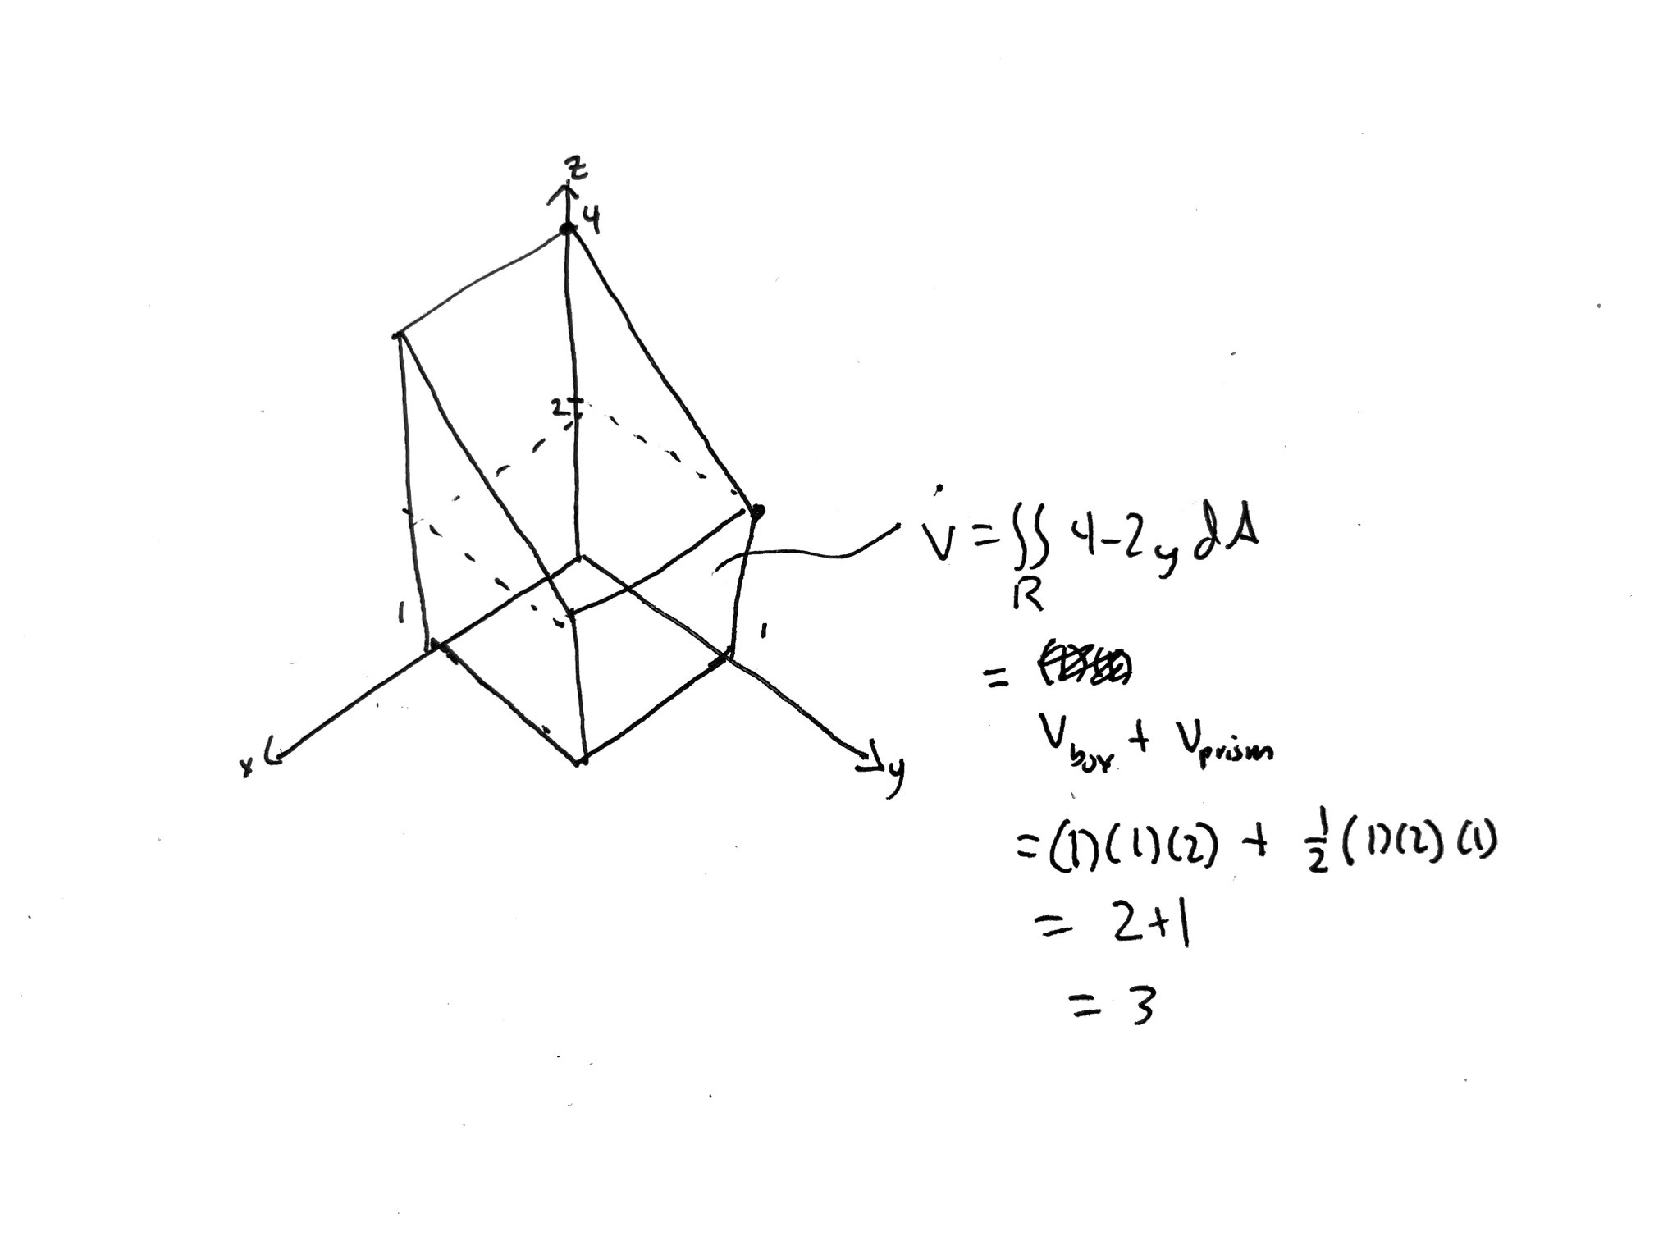
\includegraphics[scale=0.3]{ws_15_1_src.pdf}
	
	\item 
	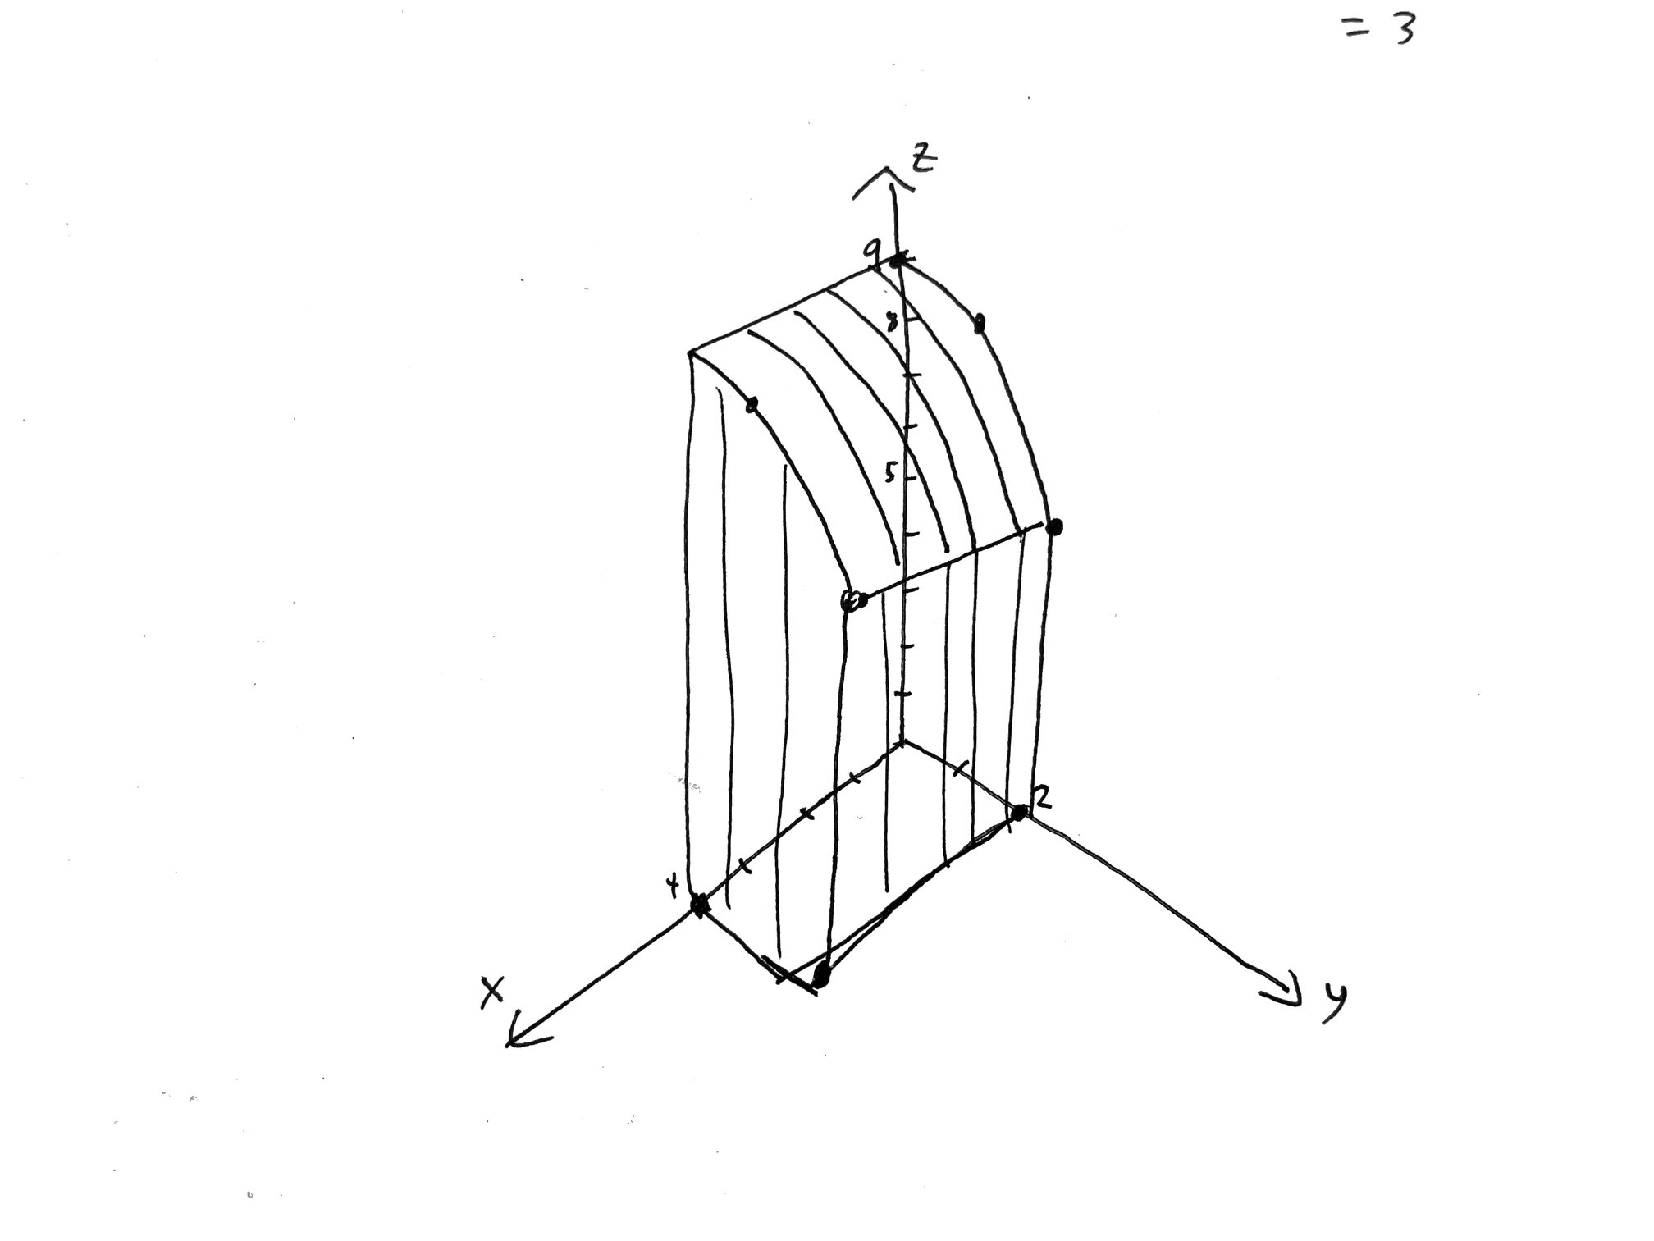
\includegraphics[scale=0.25]{ws_15_2_src.pdf}
	
	\item $9\ln(2)$
	
	\item $160/3$ cubic units.
	
		\item $e^3-4$

	\item The integrals evaluate to $\pi/4$ and $-\pi/4$ respectively.  This does not violate Fubini's theorem because this function is not continuous on $[0,1]\times[0,1]$ (it has an asymptote at $(0,0)$)
\end{enumerate}
}{}
\iftoggle{solutions}
{
Solutions go here in the same format.
}{}
